\documentclass[12pt,fleqn]{article}\usepackage{../../common}
\begin{document}
Materyel Mekaniği - 4

Potansiyel Enerji ve Denge

İlk önce denge bağlamında potansiyel enerjinin ne demek olduğunu işleyelim.

Potansiyel enerji $\Pi$ sistemin stabilitesi ile alakalıdır. Mesela alttaki
resim stabilite konusunu işleyen her ders kitabında vardır, bir kapta duran topu
aldım, yukarı doğru çıkatıp (bordo renk) aşağı bıraktım, top kabın dibine gidip
orada kalacaktır (kırmızı renk). 

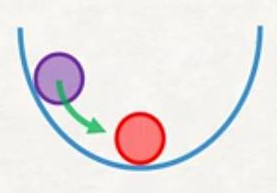
\includegraphics[width=10em]{phy_020_strs_04_01.jpg}

Yani top ilk denge konumuna dönecektir, ve o durumda potansiyel enerjisi minimum
olmuştur deriz ve bu denge stabil bir dengedir.

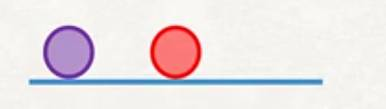
\includegraphics[width=10em]{phy_020_strs_04_02.jpg}

İkinci durumda topu orta noktada sola taşırız, top orada kalır, bu yeni
bir denge noktasıdır, $\Pi$ değişmemiştir, burada nötr bir denge vardır.

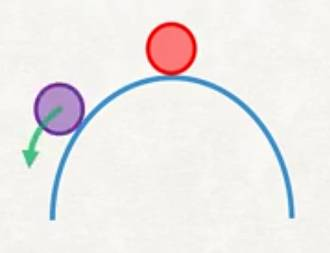
\includegraphics[width=10em]{phy_020_strs_04_03.jpg}

Üçüncü durumda ters kavisli bir yüzey var, top üst orta noktadan başlıyor
diyelim (orada durması zor olsa da), topu yine alıp sola taşıyorum, top aşağı
düşecektir. Üstteki durum potansiyel enerjisinin maksimum olduğu bir durumdur,
sistem stabil değildir. Rayleigh-Ritz yönteminin amacı (potansiyel enerjinin
minimum olduğu) stabil denge durumunu hedefleyerek bir yaklaşık çözüme
ulaşmaktır.

Bunu nasıl yaparız? Daha önce belirttiğimiz potansiyel enerjinin iki bileşeni
var, ilki sistemin toplam iç gerilim (deformasyon) enerjisi. Gerilim enerji
{\em yoğunluğu} $\overline{U}$ genel olarak bir materyelin stres-gerilim eğrisinin
altındaki alan olarak hesaplanabilir.

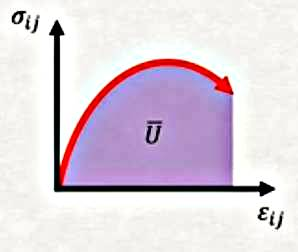
\includegraphics[width=10em]{phy_020_strs_04_04.jpg}

Mesela üstteki gibi stres $\sigma_{ij}$ ve gerilim $\epsilon_{ij}$ arasındaki
bir eğriyi düşünelim, bu eğrinin altında kalan alan, yani entegral hesabı 
gerilim enerji yoğunluğunu verir.

$$
\overline{U} = \int_{0}^{\epsilon_{ij}} \sigma_{ij} \ud \epsilon_{ij}
$$

Kolaylaştırıcı bir faktör, bizim bu derste kullanacağımız maddeler lineer
elastik, yani stres-gerilim eğrisi alttaki gibi,

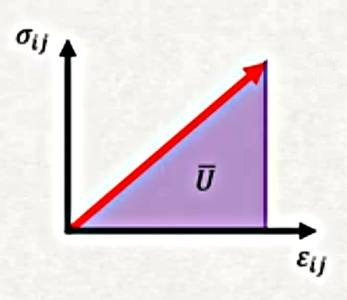
\includegraphics[width=10em]{phy_020_strs_04_05.jpg}

Bu durumda ``eğri'' yani çizgi altındaki alan basit bir üçgen hesabı,

$$
\overline{U} = \frac{1}{2} \sigma_{ij} \epsilon_{ij}
$$

Fakat bu sadece tek bir boyutu halletti, mesela üstteki örnek $e_1$ yönündeki
bir esnemeyi temsil ediyor olabilirdi, fakat 3 boyutlu ortamda elimizde daha
fazla bileşen olduğunu biliyoruz, $\sigma_{11}$ haricinde $\sigma_{22}$ var,
$\sigma_{33}$ var, $\sigma_{12}$, $\sigma_{23}$, vs.. Tüm stres/gerilim
eşleri için [2, Ders 16],

$$
\overline{U} = \frac{1}{2} \sum_{i,j=1}^{3} \sigma_{ij} \epsilon_{ij}
$$

Toplamı açarsak,

$$
= \frac{1}{2} (\sigma_{11}\epsilon_{11} + \sigma_{22}\epsilon_{22}  +
\sigma_{33}\epsilon_{33} + \sigma_{12}\epsilon_{12} + \sigma_{23}\epsilon_{23} +
\sigma_{13}\epsilon_{13} + \sigma_{33}\epsilon_{33} + \sigma_{23}\epsilon_{23} +
\sigma_{32}\epsilon_{32} )
$$

Son ifadeyi daha basitleştirmek mümkün, $\sigma$ ve $\epsilon$'un simetrik
olduğunu unutmayalım,

$$
\overline{U} = \frac{1}{2} (\sigma_{11}\epsilon_{11} + \sigma_{22}\epsilon_{22}  +
\sigma_{33}\epsilon_{33} + 2 \sigma_{12}\epsilon_{12} +
2 \sigma_{13}\epsilon_{13} + 2 \sigma_{23}\epsilon_{23} )
$$

Üsttekileri mühendislik gerilimi $\gamma_{ij} = 2 \epsilon_{ij}$ ile temsil
etmek mümkün,

$$
\overline{U} = \frac{1}{2} (\sigma_{11}\epsilon_{11} + \sigma_{22}\epsilon_{22}  +
\sigma_{33}\epsilon_{33} + \sigma_{12}\gamma_{12} +
\sigma_{13}\gamma_{13} + \sigma_{23}\gamma_{23} )
$$
 
Eksenel Yükleme (Axial Loading)

Euler-Bernoulli kiriş formülasyonu sadece bükülmenin sebep olduğu deformasyonu
hesaba kattı, bunu yaparken nötr eksen üzerindeki eksenel deformasyonu yok saydı
[3, 8.4]. Euler-Bernoulli modelini eksenel yatay deformasyonu hesaba katacak
şekilde genişletmek mümkündür, fakat, belki de bu iyi haber, ufak deformasyon
önkabulü sayesinde eksenel yük ve bükülme deformasyonları birbirinden
bağlantısız (uncoupled) hale gelir, eksenel yük sadece eksenel deformasyonu,
yatay yük sadece yatay deformasyonu etkiler.

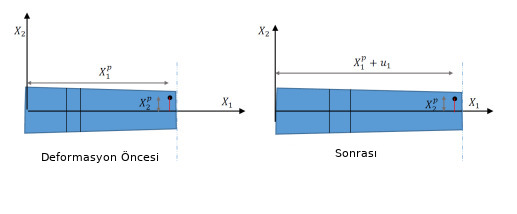
\includegraphics[width=25em]{phy_020_strs_04_06.jpg}

Diğer faraziyeler Euler-Bernoulli modeline benzer, düzlem bölümler düzlem kalır,
Poisson oranı etkileri yok sayılır, ve yatay yer değişimi $u_1$ pürüzsüz bir
fonksiyondur. Farklı bir resmi [2, Ders 15] eklersek,

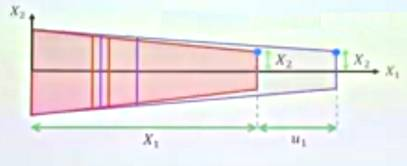
\includegraphics[width=20em]{phy_020_strs_04_08.jpg}

Bu faraziyelerle modeli oluşturalım; üstteki resme bakarsak $u_1 = u_1(X_1)$, ve
pozisyon vektör fonksiyonu olarak,

$$
x = \left[\begin{array}{c}
X_1 + u_1 \\ X_2 \\ X_3
\end{array}\right]
$$

Bu durumda yer değişim fonksiyonu

$$
u = x - X = \left[\begin{array}{c}
u_1 \\ 0 \\ 0
\end{array}\right]
$$

Hatırlarsak yaklaşık olarak gerilim tensörü

$$
\epsilon = \frac{1}{2} (\nabla u + \nabla u^T )
$$

Gradyanlar ile hesabı yaparsak sadece $\epsilon_{11}$'in sıfır olmadığını
görüyoruz,

$$
\epsilon = \left[\begin{array}{ccc}
\frac{\ud u_1}{\ud X_1} & 0 & 0 \\
0 & 0 & 0 \\
0 & 0 & 0 
\end{array}\right]
\mlabel{1}
$$

Bize gerekli diferansiyel denklemi kuvvet dengelerine bakarak ortaya
çıkartabiliriz. Şimdi kirişin $\ud X_1$ genişliğindeki ufak bir parçasına
odaklanalım,

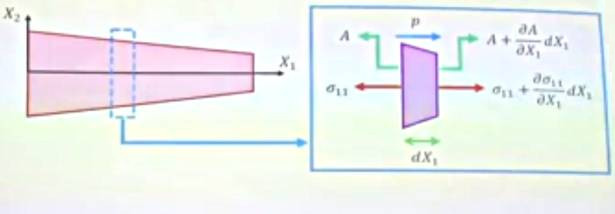
\includegraphics[width=20em]{phy_020_strs_04_07.jpg}

Bu parçanın sol ve sağındaki kuvvetlere bakarsak üstteki resim ortaya çıkar.

Oklar sola ya da sağa doğru gösterildi çünkü mesela $\sigma_{11}$ ve
$\sigma_{11} + \frac{\partial \sigma_{11}}{\partial X_1} \ud X_1$'in
birbirini dengeleyeceklerini / birbirlerine karşı ortaya çıktıklarını
biliyoruz, sağa doğru olan $p$ zaten dışarıdan uygulanan eksenel kuvvet.
$\frac{\partial \sigma_{11}}{\partial X_1}$ kullanımı $\sigma_{11}$'in
$X_1$'e oranla değişim hesabı için kullanıldı, bu oranı $X_1$'deki
olan değişimle çarpınca (örnekte $\ud X_1$) tabii ki ufak parçanın sağındaki
$\sigma_{11}$ eki ortaya çıkıyor, bunu $\sigma_{11}$'e topluyoruz.

Parçanın sol ve sağındaki alan büyüklüğü benzer şekilde, solda $A$ varsa
$A$'nin $X_1$'e oranlı değişimi çarpı $X_1$ değişimi bize parçanın sağındaki
alan büyüklük ekini veriyor. 

$X_1$ ekseni bazındaki denge denklemi o zaman alttaki gibi olur, stres hesabı
kuvvet bölü birim alan olduğu için kuvveti elde etmek için stres çarpı alan
gerekeceğini hatırlayalım, ayrıca $p$ kuvveti birim $X_1$ bazlı alınıyor,
o zaman $p \ud X_1$ kullanmak gerekir,

$$ \sum F_{X_1} = - \sigma_{11} A +
\left( \sigma_{11} + \frac{\partial \sigma_{11}}{\partial X_1} \ud X_1  \right)
\left( A + \frac{\partial A}{\partial X_1} \ud X_1  \right) + p \ud X_1 = 0
$$

Formülü açarsak

$$
-\sigma_{11} A  + \sigma_{11} A  +
\sigma_{11} \frac{\partial A}{\partial X_1} \ud X_1 +
A \frac{\partial \sigma_{11}}{\partial X_1} \ud X_1 +
\frac{\partial A}{\partial X_1} \frac{\partial \sigma_{11}}{\partial X_1} \ud X_1^2 +
p \ud X_1 = 0
$$

$\sigma_{11} A$ terimleri iptal olur,

$$
\sigma_{11} \frac{\partial A}{\partial X_1} \ud X_1 +
A \frac{\partial \sigma_{11}}{\partial X_1} \ud X_1 +
\frac{\partial A}{\partial X_1} \frac{\partial \sigma_{11}}{\partial X_1} \ud X_1^2 +
p \ud X_1 = 0
$$

$\ud X_1$ dışarı çekilir, ve sağda sıfır olduğu için iptal edilebilir,

$$
\sigma_{11} \frac{\partial A}{\partial X_1}  +
A \frac{\partial \sigma_{11}}{\partial X_1}  +
\frac{\partial A}{\partial X_1} \frac{\partial \sigma_{11}}{\partial X_1} \ud X_1 +
p  = 0
$$

Hala basitleştirme mümkün, dikkat edersek $\ud X_1$ terimini kullandık ve
ona ``çok küçük bir parça'' dedik. Bu parçayı sonsuz küçültürsek, yani
limiti alırsak, ki $\ud X \to 0$, o zaman üstteki formülde üçüncü terim
yokolur,

$$
\sigma_{11} \frac{\partial A}{\partial X_1}  +
A \frac{\partial \sigma_{11}}{\partial X_1}  
p  = 0
$$

Daha kısa bir formüle ulaştık. Fakat bize lazım olan yer değişimi, üstteki
formülde bu yok. Oraya ulaşmaya çalışalım. Dikkat edersek üstteki formülde
ilk iki terim sanki Calculus'ta çarpım kuralının açılmış haline benziyor,
o zaman o kuralı ters yönde işletirsek, yani gruplama amaçlı geriye gidersek,

$$
\frac{\partial }{\partial X_1} (\sigma_{11} A ) + p = 0
$$

Şimdi $\sigma_{11} = E \epsilon_{11}$ formülünü hatırlayalım, bu nereden geldi?
Elimizde bir tekeksenel yük var, o zaman en baz stres-gerilme ilişkisi geçerli
olur, yerine koyarsak,

$$
\frac{\partial }{\partial X_1} (E \epsilon_{11} A ) + p = 0
$$

Peki $\epsilon_{11}$ nedir? Bu büyüklüğü (1)'de gördük, $\epsilon$'un tek sıfır
olmayan öğesi $\epsilon_{11}$ ve orada $\frac{\ud u_1}{\ud X_1}$ değeri
var. Bunu üstteki formüle koyalım,

$$
\frac{\partial }{\partial X_1} \left( E A \frac{\ud u_1}{\ud X_1} \right) + p = 0
$$

Böylece içinde yer değişimi içeren bir formül elde etmiş oldum, $u_1$ yer
değişimidir.

Bu denklemi artık çözüm için kullanabiliriz. Tasarımcı olarak biz Young'in
Genliği $E$'yi biliriz, kirişin herhangi bir noktasındaki satıhsal alan $A$'yi
biliriz, kirişe uygulanan yük $p$'yi biliriz, tüm bunları kullanarak yer değişim
$u_1$'i üstteki formülle bulabiliriz. Tek bilinmeyen $u_1$ çünkü.

Şimdi bu noktada bazı püf noktalar ortaya çıkıyor; çünkü eğer $E,A$ büyüklükleri
$X_1$'in fonksiyonu iseler çözüm daha karmaşık hale gelebilir çünkü üstteki
formülde dış türev $X_1$'e göre. Fakat şimdiye kadar bu derste $X_1$'e bağlı bir
$E$ görmedik, yani Young'in Genliği kirişin her noktasında aynı, özetle sabit.
Sabit ise $E$ diferansiyelin dışına alınabilir. $A$ aynı şekilde. Eğer $A$
değişken ise o zaman Calculus çarpım kuralı uygularız.

O zaman iki senaryo şöyle olabilir, $E$ sabit ama $A$ değil,

$$
E \frac{\partial A}{\partial X_1} \frac{\partial u_1}{\partial X_1} +
EA \frac{\partial^2 u_1}{\partial X_1} + p = 0
$$

Hem $E$ hem $A$ sabit,

$$
E A \frac{\partial^2 u_1}{\partial X_1} + p = 0
$$

Üç Boyutta Eşyönlü (Isotropic) Stres-Gerinim İlişkisi 

Şimdi bir kütleye uygulanan stres sonucu ortaya çıkan gerinimi üç boyut için
formülize edeceğiz [6, sf. 871]. Maddenin lineer elastik ve eşyönlü olduğu farz
edilecek, yani uygulanan bir stres farklı yönlerde etkilere sebep olursa bu etki
her yönde eşit şekilde ortaya çıkacak. Aradığımız formül Hooke Kanunu'nun üç
boyutlu hali, buna bazı kaynaklar (listelenen şartlar için) Genelleştirilmiş
Hooke Kanunu ismi de verebiliyor.

Bir gövdeyi her eksen üzerinden $\sigma_x$, $\sigma_y$, $\sigma_z$ streslerine
tabi tutacağız ve sonuçları inceleyeceğiz. Mesela temel Hooke Kanunu $\sigma = E
\epsilon$'den yola çıkarak $\epsilon_x^x = \sigma_x / E$ diyebiliriz,
$\epsilon_x^x$ büyüklüğündeki üstsimge gerinimin $x$ stresi sebebiyle olduğunu
söylüyor, diğerleri de olacak.

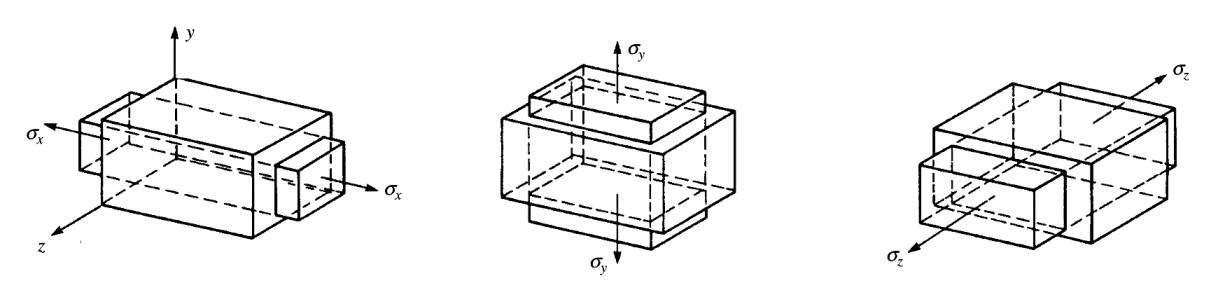
\includegraphics[width=35em]{phy_020_strs_00_10.jpg}

Fakat stres-gerinim ilişkisi sadece tek eksenle kısıtlı değil. Bir eksende stres
uyguladığımızda bunun diğer eksenler üzerinde de etkileri olacaktır.  Çünkü
madde bir yöne uzayıp şekil değiştirir fakat diğer eksenlerde ufalma olacağı
için o eksenlerde eksi yönde gerinim olur.

Mesela üstte ortadaki resmi düşünürsek, $\sigma_y$ stresi uygulandığında $x$
yönünde bir negatif gerinim olur, çünkü madde o eksen bağlamında içe doğru
daralır, şekil değiştirir, bunu formül

$$
\epsilon_x^y =  \frac{- v \sigma_y}{E}
$$

ile gösterebiliriz ki $v$ Poisson oranı. Dikkat $y$ yönündeki stresin etkisi
sadece $E$ sabiti ile değil $v/E$ sabiti ile $y$ eksenine yansıyor. Bu normal
olmalı çünkü bir eksene direk uygulanan stres ve onun aynı eksende yol açtığı
gerinim diğer eksenlerdeki yan etki gibi görülebilecek gerinimler ile aynı
olamaz.

Benzer şekilde $z$ stresinin yol açtığı gerinim

$$
\epsilon_x^z =  \frac{- v \sigma_z}{E}
$$

Tum bu gerinimleri toplarsak $x$ eksenindeki toplam gerinim elde edilir,

$$
\epsilon_x = \epsilon_x^x + \epsilon_x^y + \epsilon_x^z
$$

$$
= \frac{\sigma_x}{E} - \frac{v \sigma_y}{E} - \frac{v \sigma_z}{E} 
$$

Benzer şekilde $y$ ve $z$ yönündeki gerinimler de elde edilebilir,

$$
\epsilon_y = \frac{\sigma_y}{E} - \frac{v \sigma_x}{E} - \frac{v \sigma_z}{E} 
$$

$$
\epsilon_z = \frac{\sigma_z}{E} - \frac{v \sigma_x}{E} - \frac{v \sigma_y}{E} 
$$

Son üç denklemi birleştirip stresler solda olacak şekilde düzenlersek,

$$
\sigma_x = \frac{E}{(1+v)(1-2v)} [\epsilon_x (1-v) + v \epsilon_y + v \epsilon_z ]
$$

$$
\sigma_y = \frac{E}{(1+v)(1-2v)} [ v \epsilon_x + \epsilon_y (1-v) + v \epsilon_z  ]
$$

$$
\sigma_z = \frac{E}{(1+v)(1-2v)} [v \epsilon_x + v \epsilon_y + \epsilon_z (1-v)  ]
$$

Ayrıca normal stresler için kullanılan Hooke Kanunu $\sigma = E \epsilon$ benzer
bir şekilde kaykılma stresi ve kaykılma gerinimi için de geçerlidir, ama sabit
$E$ yerine $G$ kullanılır,

$$
\tau = G \gamma
$$

$G$ sabitine Kaykılma Genliği (Shear Modulus) ismi veriliyor. 0 zaman üç boyutta
ortaya çıkabilecek üç kaykılma stresi

$$
\tau_{xy} = G \gamma_{xy} \qquad 
\tau_{yz} = G \gamma_{yz} \qquad 
\tau_{zx} = G \gamma_{zx}
$$

$G$ ile $E$ arasında bir ilişki var, bu formül

$$
G = \frac{E}{2(1+v)}
$$

Bu formülün türetilmesi için [7, sf. 70]'e bakılabilir.

Şimdi üstteki tüm formülleri matris formunda bir araya koyabiliriz,

$$
\left[\begin{array}{c}
\sigma_x \\ \sigma_y \\ \sigma_z \\ \tau_{xy} \\ \tau_{yz} \\ \tau_{zx}
\end{array}\right] =
\frac{E}{(1+v)(1-2v)}
\left[\begin{array}{cccccc}
1-v &  v  &  v  &            0      &               0  &  0  \\
 v  & 1-v &  v  &            0      &               0  &  0  \\
 v  &  v  & 1-v &            0      &               0  &  0  \\
 0  &  0  &  0  & \dfrac{1-2v}{2}   &               0  &  0  \\
 0  &  0  &  0  &            0      &  \dfrac{1-2v}{2} &  0  \\
 0  &  0  &  0  &            0      &               0  &  \dfrac{1-2v}{2} 
\end{array}\right]
\left[\begin{array}{c}
\epsilon_x \\ \epsilon_y \\ \epsilon_z \\ \gamma_{xy} \\ \gamma_{yz} \\ \gamma_{zx}
\end{array}\right]
$$

Matrisin sol alt kısmı doldurulmadı orası simetri sebebiyle sağ üst kısım ile
aynı.

Eğer gerinim değişkenlerini eşitliğin solunda stresleri sağda tutmak istersek,
üstteki matrisin tersini bulmamız lazım [8, sf. 161], sembolik ters alma
işlemini \verb!sympy! ile yapabiliriz,

\begin{minted}[fontsize=\footnotesize]{python}
import sympy as sym
E, v = sym.symbols('E v')
matrix = E/((1+v)*(1-2*v))*sym.Matrix([[1-v,v,v,0,0,0],
                     [v,1-v,v,0,0,0],
		     [v,v,1-v,0,0,0],
		     [0,0,0,(1-2*v)/2,0,0],
                     [0,0,0,0,(1-2*v)/2,0],
		     [0,0,0,0,0,(1-2*v)/2]])
sym.latex(matrix.inv())
\end{minted}


$$
\left[\begin{matrix}\dfrac{1}{E} & - \dfrac{v}{E} & - \dfrac{v}{E} & 0 & 0 & 0\\- \dfrac{v}{E} & \dfrac{1}{E} & - \dfrac{v}{E} & 0 & 0 & 0\\- \dfrac{v}{E} & - \dfrac{v}{E} & \dfrac{1}{E} & 0 & 0 & 0\\0 & 0 & 0 & \dfrac{2 v + 2}{E} & 0 & 0\\0 & 0 & 0 & 0 & \dfrac{2 v + 2}{E} & 0\\0 & 0 & 0 & 0 & 0 & \dfrac{2 v + 2}{E}\end{matrix}\right]
$$

Bir basitleştirme daha yapılabilir, bunu kendimiz görebiliyoruz, $1/E$ dışarı
çekelim, hepsini bir araya koyalım,

$$
\left[\begin{array}{c}
\epsilon_x \\ \epsilon_y \\ \epsilon_z \\ \gamma_{xy} \\ \gamma_{yz} \\ \gamma_{zx}
\end{array}\right] =
\frac{1}{E}
\left[\begin{array}{cccccc}
1 & -v & -v & 0 & 0 & 0 \\
-v & 1 & -v & 0 & 0 & 0 \\
-v & -v & 1 & 0 & 0 & 0 \\
0 & 0 & 0 & 2(1+v) & 0 & 0 \\
0 & 0 & 0 & 0 & 2(1+v) & 0 \\
0 & 0 & 0 & 0 & 0 & 2(1+v)
\end{array}\right]
\left[\begin{array}{c}
\sigma_x \\ \sigma_y \\ \sigma_z \\ \tau_{xy} \\ \tau_{yz} \\ \tau_{zx}
\end{array}\right]
$$

Düzlem Stresi (Plane Stres)

Eğer bir gövde sadece iki boyutta strese tabi tutuluyorsa bu gövdenin ``düzlem
stresi'' durumunda olduğu söylenir [3, sf. 70]. Bu tür stres / gerinimde
$\sigma_z = \tau_{xz} = \tau_{yz} = 0$'dir yani üçüncü boyut $z$ eksenine dönük
hiçbir aksiyon yoktur. Bu durumda Genel Hooke Kanunu alttaki üç denkleme
indirgenebilir,

$$
\sigma_x = \frac{1}{E} (\sigma_x - v \sigma_y )
$$

$$
\sigma_y = \frac{1}{E} (\sigma_y - v \sigma_x )
$$

$$
\gamma_{xy} = \frac{1}{G} \tau_{xy}
$$

Üç boyutlu durumda olduğu gibi üstteki formülleri matris formunda
gösterebiliriz,

$$
\left[\begin{array}{c}
\epsilon_{x} \\ \epsilon_{y} \\ \gamma_{xy}
\end{array}\right] =
\frac{1}{E}
\left[\begin{array}{ccc}
1 & -v & 0 \\
-v & 1 & 0 \\
0 & 0 & 2(1+v)
\end{array}\right]
\left[\begin{array}{c}
\sigma_x \\ \sigma_y \\ \tau_{xy}
\end{array}\right]
$$

Yine bir yer değiştirme işlemi yapılabilir, üstteki matrisin tersini alırsak
stresler sola geçer, 

$$
\left[\begin{array}{c}
\sigma_x \\ \sigma_y \\ \tau_{xy}
\end{array}\right] = 
\frac{E}{(1-v)^2}
\left[\begin{array}{ccc}
1 & v & 0 \\ v & 1 & 0 \\ 0 & 0 & \dfrac{(1-v)}{2}
\end{array}\right]
\left[\begin{array}{c}
\epsilon_{x} \\ \epsilon_{y} \\ \gamma_{xy}
\end{array}\right] 
$$

Bazı formülasyonlarda üstteki matrisin çarpan sabitin böleninde $(1+v)$
görülebiliyor, bu durumda $(1-v)^2=(1+v)(1-v)$ olduğunu hatırlayalım, ve ona
göre matrisin tüm öğeleri $(1-v)$ ile bölünmüş olacaktır, farketmez, her iki
form da aynı sonucu verir.

Elastiklik Denge Denklemleri

Gerinme (yer değişim) ve stres arasındaki ilişki gösterildi, şimdi tüm
kuvvetlerin arasındaki denge denklemlerine bakalım. Eğer dışarıdan her eksen
üzerinde, X, Y, Z kuvvetleri uygulansa, ya da uygulanmasa bile, mevcut direk
stresler $\sigma$ ve yüzeylere paralel giden kaykılma stresleri $\tau$
arasındaki denge ilişkisi ne olurdu?

Önce idealize edilmiş her kenarı ufak $\ud x$, $\ud y$, $\ud z$ boyutlarında
olan bir küp düşünelim, küpün kenarlarına $X,Y,Z$ kuvvetleri uygulanıyor.

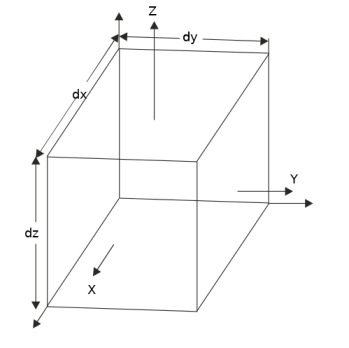
\includegraphics[width=10em]{equilibrium_stress2.jpg}

Bu kuvvetlerin ortaya çıkardığı direk ve kaykılma stresleri alttaki gibi
gösterilebilir.

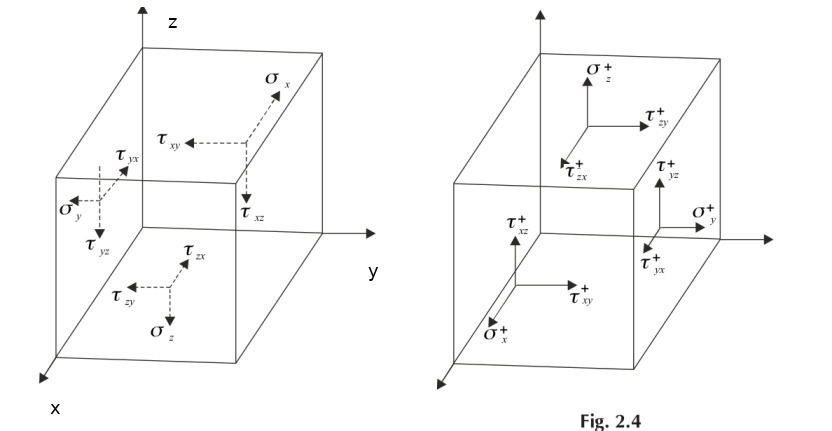
\includegraphics[width=30em]{equilibrium_stress1.jpg}

Küpün kordinate eksenlerine paralel olan yüzü nötr diğerleri ``artı yüzleri''
olarak simgelendirildi, mesela üst sağdaki resimde okuyucuya yakın olan yüzden
dışarı doğru çıkan stres $\sigma_x^+$ sembolü, aynı yüzdeki kaykılma stresleri
benzer şekilde artı işaretini alıyor, $x$ eksenine doğru / dik oldukları için
ilk altsembolleri $x$, paralel ilerledikleri eksen ikinci alt sembol, mesela sağ
yönünü gösteren kaykılma stresi $\tau_{xy}^+$. Artı yüzün tam karşısındaki direk
stres $\sigma_x$, onda artı işareti yok.

Eğer bir denge formülü bulmak istiyorsak her yüz için bu eşitlikleri ayrı ayrı
kurabiliriz. Mesela $x$ ekseni ile başlayalım, iki stresten bahsettik zaten,
$\sigma_x^+$ ve $\sigma_x$. Fakat bu yönde yani $x$ ekseni boyunca etki eden
stresler sadece onlar değil, bu yönde olan kaykılma stresleri de var. İşaret
edilen yön ikinci altsembol demiştik, orada $x$ diyen tüm kaykılma streslerini
kolayca bulabiliriz, $\tau_{yx}$, $\tau_{zx}$, $\tau_{yx}^+$, $\tau_{zx}^+$.

Denge formülünden önce artı yüzleri hakkında bir ek bilgi daha verelim, bu
yüzlerin stresini karşısındaki stresi baz alarak formülize edebiliriz,
yani $\sigma_x^+$ formülü $\sigma_x$ bazlı gösterilebilir, bunu kısmı türev
ile yaparız, 

$$
\sigma_x^+ = \sigma_x + \frac{\partial \sigma_x}{\partial x} \ud x
$$

Türev bağlamında üstteki akla yatkın olmalı, eğer $\partial \sigma_x / \partial x$
bir değişim oranınıdır, onu ufak değişim miktarı $\ud x$ ile çarpıp
$\sigma_x$'e eklersek $\sigma_x^+$ elde edebiliriz. Benzer mantığı tüm artı
yüzlerdeki stresler için kullanabiliriz.

Bir ek konu daha, stres daha önce belirtiğimiz gibi kuvvet / alan hesabıdır,
fakat denge formülü kuvvetler üzerinden yapılacak o zaman bildiğimiz, bulduğumuz
her stres büyüklüğünü onun etki ettiği alan ile çarpmamız gerekir, ki böylece
kuvvet elde edelim ve bu kuvvetleri toplayarak sıfır eşitleyip denge formülünü
bulalım. Yine $x$ örneği, $\sigma_x$'in etki ettiği alan $\ud y \ud z$ alanıdır.

Devam edelim, $x$ ile başlayalım, o yöndeki denge için $x$ yönündeki tüm
kuvvetleri toplamak gerekir, artı yüzdeki kuvveti pozitif yapacağız (bunu
hatırlaması kolay), tersini gösteren kuvvet ise negatif olacak, $X$ gövdeye
uygulanan birim hacimdeki dış kuvvettir, o zaman tüm $x$ toplamı

$$
  \sigma_x^+ \ud y \ud z - \sigma_x \ud y \ud z +
  \tau_{yx}^+ \ud x \ud z - \tau_{yx} \ud x \ud z +
  \tau_{zx}^+ \ud x \ud y - 
$$
$$
  \tau_{zx} \ud x \ud y +   X \ud x \ud y \ud z = 0
$$

Artı yüzlerdeki stresleri diğer yüz bağlamında temsil edebiliriz demiştik, bunu
yapalım,

$$
(\sigma_x  + \dfrac{\partial \sigma_x}{\partial x} \ud x )\ud y \ud z - \sigma_x \ud y \ud z +
(\tau_{yx}  + \dfrac{\partial \tau_{yx}}{\partial y} \ud y ) \ud x \ud z -
\tau_{yx} \ud x \ud z +
$$
$$
(\tau_{zx}  + \dfrac{\partial \tau_{zx}}{\partial z} \ud z ) \ud x \ud y - \tau_{zx} \ud x \ud y +
X \ud x \ud y \ud z = 0
$$

Basitleştirip her şeyi $\ud x \ud y \ud z$ ile bölersek,

$$
\frac{\partial \sigma_x}{\partial x} + 
\frac{\partial \tau_{yx}}{\partial y} + 
\frac{\partial \tau_{zx}}{\partial z} + X = 0
$$

Benzer hesabı $y$, $z$ icin yaparsak,

$$
\frac{\partial \tau_{xy}}{\partial x} + 
\frac{\partial \sigma_y}{\partial y} + 
\frac{\partial \tau_{zy}}{\partial z} + Y = 0
$$

$$
\frac{\partial \tau_{xz}}{\partial x} + 
\frac{\partial \tau_{yz}}{\partial y} + 
\frac{\partial \sigma_z}{\partial z} + Z = 0
$$

Kaynaklar

[1] Petitt, {\em Intro to the Finite Element Method}, University of Alberta,
    \url{https://www.youtube.com/watch?v=2iUnfPRk6Ro&list=PLLSzlda_AXa3yQEJAb5JcmsVDy9i9K_fi}

[2] Petitt, {\em Intro to the Continuum Mechanics}, University of Alberta,
    \url{https://www.youtube.com/playlist?list=PLLSzlda_AXa3N5jaDART7kimBlYz1dFnX}

[3] Adeeb, {\em Introduction to Solid Mechanics}
    \url{https://engcourses-uofa.ca/books/introduction-to-solid-mechanics/}

[4] Bhavikatti, {\em Finite Element Analysis}    
    
[5] Khennane, {\em Introduction to Finite Element Analysis Using MATLAB and Abaqus}

[6] Logan, {\em A First Course in the FEM, 5th Ed}

[7] Craig, {\em Mechanics of Materials, Third Edition}

[8] Khennane, {\em Introduction to Finite Element Analysis using Matlab and Abaqus}

\end{document}
